% !TeX root = ../../infdesc.tex

\begin{exercise}
\label{exExamplesOfPropositions}
Think of an example of (a) a true proposition; (b) a false proposition; and (c) a proposition whose truth value you don't know.
\end{exercise}

\begin{solutions*}
  \fixlistskip
  \begin{enumerate}[(a)]
  \item $2$ is an even number.
  \item $2$ is an odd number.
  \item Every even integer greater than two can be expressed as the sum of two positive prime numbers. [This is \textit{Goldbach's conjecture}, proposed in 1742 by Christian Goldbach. It a famous example of an extant \textit{open problem} in mathematics. Will you be the one to solve it?]
  \end{enumerate}
\end{solutions*}


\begin{exercise}
\label{exFloorCeilingOfNonInteger}
Suppose that $x$ is a real number that is not an integer. Prove that $\ceil{x} = \floor{x} + 1$.
\end{exercise}

\begin{solutions*}
Set $n = \floor{x}$. Then $n \le x < n+1$ by definition of floor. Since $x$ is not an integer and $n$ is, we have $n < x$; but then $n<x<n+1$, and so $(n+1)-1 < x \le n+1$. This inequality demonstrates that $n+1$ is the ceiling of $x$, and so $\ceil{x} = n+1 = \floor{x} + 1$, as required.
\end{solutions*}

\begin{exercise}
Suppose that $x$ is a real number. Prove that $\floor{-x} = -\ceil{x}$ and $\ceil{-x} = -\floor{x}$.
\end{exercise}

\begin{solutions*}
Set $n = \floor{-x}$. By definition of floor we have $n \le -x < n+1$. Multiplying through by $-1$ gives $-n \ge x > -(n+1)$, or equivalently $-n-1 < x \le -n$. Thus $-n$ satisfies the definition of being the ceiling of $x$, so that $\ceil{x} = -n = -\floor{-x}$. Hence $\floor{-x} = -\ceil{x}$, as required.

Now set $m = \ceil{-x}$. By definition of ceiling we have $m-1 < -x \le m$. Multiplying through by $-1$ and rearranging gives $-m \le x < -m+1$. Thus $\floor{x} = -m = -\ceil{-x}$, and so $\ceil{-x} = -\floor{x}$, as required.
\end{solutions*}

\begin{exercise}
\label{exRationalNumbersAreAField}
Complete the proof of \Cref{thmRationalNumbersAreAField}.
\end{exercise}

\begin{solutions*}
Let $a,b,c,d$ be integers, with $b \ne 0$ and $d \ne 0$, such that $x=\dfrac{a}{b}$ and $y=\dfrac{c}{d}$; we know $a,b,c,d$ exist by the definition of what it means for $x$ and $y$ to be rational. Then:
\begin{itemize}
\item $x-y = \dfrac{a}{b} - \dfrac{c}{d} = \frac{ad-bc}{bd}$;
\item $xy = \dfrac{a}{b} \times \dfrac{c}{d} = \dfrac{ac}{bd}$; and
\item If $y \ne 0$, then $c \ne 0$ (since if $c=0$ then $y=\dfrac{c}{d}=\dfrac{0}{d}=0$), and so $\dfrac{x}{y} = \dfrac{a/b}{c/d} = \dfrac{ad}{bc}$.
\end{itemize}
The expressions on the right-hand side of each of the above chains of equations is a fraction of two integers, with a nonzero integer in the denominator, and so the numbers $x+y$, $x-y$, $xy$ and $\dfrac{x}{y}$ are all rational.%
\end{solutions*}

\begin{exercise}
\label{exElementsOfNumberSets}
Determine the truth values of the following propositions.
\begin{multicols}{3}
\begin{enumerate}[(a)]
\item $2 \in \Nat$
\item $-2 \in \Nat$
\item $-2 \in \Rat$
\item $\dfrac{2}{5} \in \Int$
\item $\dfrac{\sqrt{8}+\sqrt{2}}{\sqrt{8}-\sqrt{2}} \in \Rat$
\item $\pi^{\pi} \in \Rat$
\item $\sqrt{-7} \in \Real$
%\item $\sqrt{-7} \in \Cplx$
\item\label{itmNElementOfZ} $\Nat \in \Int$
\end{enumerate}
\end{multicols}
\end{exercise}

\begin{solutions*}
  \fixlistskip
\begin{enumerate}[(a)]
\item $2 \in \Nat$ is true, since it is a nonnegative whole number and can be used for counting (for example, I have $2$ eyes).
\item $-2 \in \Nat$ is false, since $-2 < 0$ but all natural numbers are nonnegative.
\item $-2 \in \Rat$ is true, since $-2 = \dfrac{-2}{1}$, which is an integer divided by a nonzero integer.
\item $\dfrac{2}{5} \in \Int$ is false, since $0<\dfrac{2}{5}<1$, meaning that $\dfrac{2}{5}$ is strictly between two consecutive integers.
\item $\dfrac{\sqrt{8}+\sqrt{2}}{\sqrt{8}-\sqrt{2}} \in \Rat$ is true: note that $\sqrt{8} = 2\sqrt{2}$, so cancelling the common factor of $\sqrt{2}$ from the numerator and denominator reveals that this number is equal to $\dfrac{2+1}{2-1} = \dfrac{3}{1}$, which is an integer divided by a nonzero integer.
\item $\pi^{\pi} \in \Rat$\dots{} OK, sorry, this is (kind of) a trick question. Whether or not $\pi^{\pi}$ is rational is an open problem.
\item $\sqrt{-7} \in \Real$ is false: the square of every real number is nonnegative, but whatever $\sqrt{-7}$ actually \textit{is},\footnote{$\sqrt{-7}$ is an example of a \textit{complex number}, which is a topic for another time.} it presumably satisfies $\sqrt{-7}^2=-7$, which is negative.
%\item $\sqrt{-7} \in \Cplx$ is true, with a caveat: $-7$ actually has two complex square roots, namely $\sqrt{7}i$ and $-\sqrt{7}i$, and it is not immediately obvious which of these the expression `$\sqrt{-7}$' refers to. But both $\sqrt{7}i$ and $-\sqrt{7}i$ are indeed complex numbers.
\item $\Nat \in \Int$ might appear true at first sight, since every natural number is indeed an integer. However, $\Nat$ is \textit{the set of all natural numbers}, which is a set, not an integer, and so the proposition $\Nat \in \Int$ is false.
\end{enumerate}
\end{solutions*}


\begin{exercise}
\label{exNotationsInvolvingBrackteN}
Let $A = \setb{x \in [10]}{x \text{ is a power of } 2}$, let $B = \setb{2^x}{x \in [10]}$ and let $C = \{ {-99}, {-97}, \dots{}, 95, 97, 99 \}$.
\begin{enumerate}[(a)]
\item Find a list notation expression for $A$.
\item Find a list notation expression for $B$.
\item Find a set-builder notation expression for $C$ that involves a set of the form $[n]$ for some $n \in \mathbb{N}$.
\end{enumerate}
\end{exercise}

\begin{solutions*}
\fixlistskip
\begin{enumerate}[(a)]
\item The elements of $[10]$ are the natural numbers that are less than $10$, and those that are also powers of $2$ are $2^0=1$, $2^1=2$, $2^2=4$ and $2^3=8$; therefore $A = \{ 1, 2, 4, 8 \}$.
\item $B$ is obtained by raising $2$ to the powers given by the elements of $[10]$; thus
\[ B = \{ 2^0, 2^1, \dots, 2^9 \} = \{ 1, 2, 4, 8, 16, 32, 64, 128, 256, 512 \} \]
\item An integer is an element of $C$ precisely if its absolute value is odd and less than $100$; thus
\[ C = \Bigsetb{n \in \mathbb{Z}}{|n| \in [100] \text{ and } n \text{ is odd}} \]
Another perspective is that by adding $99$ to the elements of $C$ and then dividing by $2$ we obtain the numbers $0, 1, 2, \dots, 99$, which are the elements of $[100]$; thus we obtain the element of $C$ by reversing these operations, i.e.\ taking the elements of $[100]$, multiplying them by $2$ and then subtracting $99$. Thus
\[ C = \setb{2x-99}{x \in [100]} \]
\end{enumerate}
\end{solutions*}


\begin{exercise}
\label{exIntervalDiagrams}
Express each of the sets illustrated below using the most appropriate notation. A filled circle $\bullet$ indicates that a point is included in the set, whereas a hollow circle $\circ$ indicates that an end-point is not included in the interval.

\begin{enumerate}[(a)]
\item
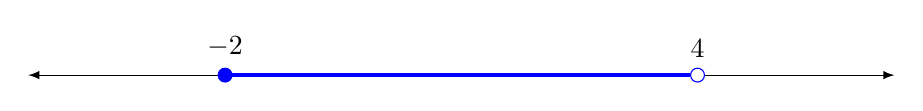
\begin{tikzpicture}
\draw[latex-latex] (-5.5,0) -- (5.5,0);
\draw[line width=1.5pt, color=blue] (-3,0) -- (3,0);
\filldraw[blue](-3,0)circle[radius=2.5pt];
\filldraw[white](3,0)circle[radius=2.5pt];
\draw[blue](3,0)circle[radius=2.5pt];
\node[at={(-3,3pt)},above]{$-2$};
\node[at={(3,3pt)},above]{$4$};
\end{tikzpicture}

\item
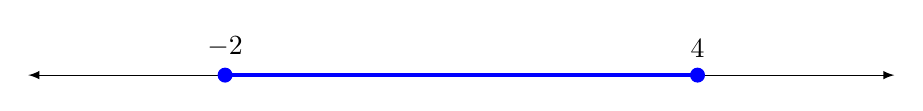
\begin{tikzpicture}
\draw[latex-latex] (-5.5,0) -- (5.5,0);
\draw[line width=1.5pt, color=blue] (-3,0) -- (3,0);
\filldraw[blue](-3,0)circle[radius=2.5pt];
\filldraw[blue](3,0)circle[radius=2.5pt];
\node[at={(-3,3pt)},above]{$-2$};
\node[at={(3,3pt)},above]{$4$};
\end{tikzpicture}

\item
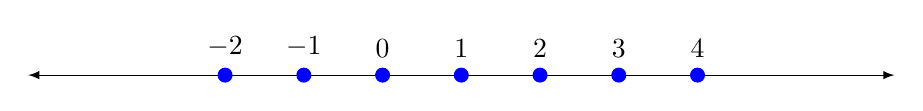
\begin{tikzpicture}
\draw[latex-latex] (-5.5,0) -- (5.5,0);
\filldraw[blue](-3,0)circle[radius=2.5pt];
\filldraw[blue](-2,0)circle[radius=2.5pt];
\filldraw[blue](-1,0)circle[radius=2.5pt];
\filldraw[blue](0,0)circle[radius=2.5pt];
\filldraw[blue](1,0)circle[radius=2.5pt];
\filldraw[blue](2,0)circle[radius=2.5pt];
\filldraw[blue](3,0)circle[radius=2.5pt];
\node[at={(-3,3pt)},above]{$-2$};
\node[at={(-2,3pt)},above]{$-1$};
\node[at={(-1,3pt)},above]{$0$};
\node[at={(0,3pt)},above]{$1$};
\node[at={(1,3pt)},above]{$2$};
\node[at={(2,3pt)},above]{$3$};
\node[at={(3,3pt)},above]{$4$};
\end{tikzpicture}


\item
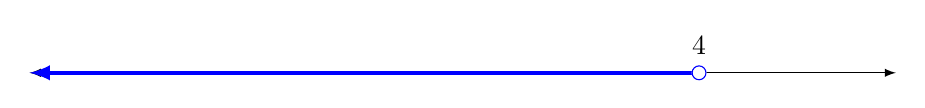
\begin{tikzpicture}
\draw[latex-latex] (-5.5,0) -- (5.5,0);
\draw[latex-, line width=1.5pt, color=blue] (-5.5,0) -- (3,0);
\filldraw[white](3,0)circle[radius=2.5pt];
\draw[blue](3,0)circle[radius=2.5pt];
\node[at={(3,3pt)},above]{$4$};
\end{tikzpicture}

\item 
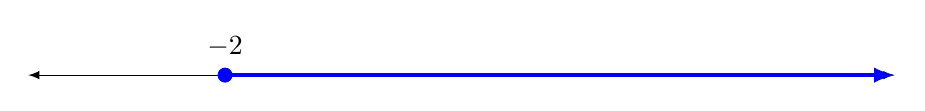
\begin{tikzpicture}
\draw[latex-latex] (-5.5,0) -- (5.5,0);
\draw[-latex, line width=1.5pt, color=blue] (-3,0) -- (5.5,0);
\filldraw[blue](-3,0)circle[radius=2.5pt];
\node[at={(-3,3pt)},above]{$-2$};
\end{tikzpicture}

\item 

\begin{tikzpicture}
\draw[latex-latex] (-5.5,0) -- (5.5,0);
\draw[latex-latex, line width=1.5pt, color=blue] (-5.5,0) -- (5.5,0);
\end{tikzpicture}
\end{enumerate}%
\end{exercise}

\begin{solutions*}
\fixlistskip%
\begin{enumerate}[(a)]
\item $[{-2},4)$
\item $[{-2},4]$
\item $\{ {-2}, {-1}, 0, 1, 2, 3, 4 \}$ --- note that interval notation $[{-2},4]$ is \textit{not} appropriate in this case, since the non-integer real numbers between $-2$ and $5$ are not elements of the set.
\item $({-\infty},4)$
\item $[{-2},\infty)$
\item You might be tepmted to write $({-\infty},\infty)$ for this one, and that is generally considered acceptable, but it can even more concisely be expressed simply as $\Real$.
\end{enumerate}
\end{solutions*}


\begin{exercise}
Find the binary, ternary, octal, decimal, hexadecimal and base-$36$ expansions of the number $21127$, using the letters $\mathrm{A}$--$\mathrm{F}$ as additional digits for the hexadecimal expansion (representing the numbers $10$--$15$, respectively), and the letters $\mathrm{A}$--$\mathrm{Z}$ as additional digits for the base-$36$ expansion.
\end{exercise}


\begin{exercise}
\label{exOneDividesEveryIntegerDividesZero}
Prove that $1$ divides every integer, and that every integer divides $0$.
\end{exercise}

\begin{exercise}
\label{exDivisibilityIsLinear}
Let $a,b,d \in \Int$. Suppose that $d$ divides $a$ and $d$ divides $b$. Given integers $u$ and $v$, prove that $d$ divides $au+bv$.
\end{exercise}


\begin{exercise}
Prove that if an integer $a$ leaves a remainder of $r$ when divided by an integer $b$, then $a$ leaves a remainder of $r$ when divided by $-b$.
\end{exercise}


\begin{exercise}
Find the base-$17$ expansion of $408\,735\,787$ and the base-$36$ expansion of $1\,442\,151\,747$.
\end{exercise}


\begin{exercise}
Let $r$ be a rational number and let $a$ be an irrational number. Prove that it is possible that $ra$ be rational, and it is possible that $ra$ be irrational.
\end{exercise}


\begin{exercise}
Interpret the operations of subtraction and division as geometric transformations of the real number line.
\end{exercise}